\documentclass[conference]{IEEEtran}
\IEEEoverridecommandlockouts
% The preceding line is only needed to identify funding in the first footnote. If that is unneeded, please comment it out.
\usepackage{cite}
\usepackage{breqn}
\usepackage{algorithm2e}
\usepackage{amsmath,amssymb,amsfonts}
\usepackage{algorithmic}
\usepackage{graphicx}
\usepackage{textcomp}
\usepackage{xcolor}
\usepackage{verbatim}
\usepackage{mathtools}
\DeclarePairedDelimiter\abs{\lvert}{\rvert}%
\DeclarePairedDelimiter\norm{\lVert}{\rVert}%
\newcommand{\RomanNumeralCaps}[1]{\MakeUppercase{\romannumeral #1}}
% Swap the definition of \abs* and \norm*, so that \abs
% and \norm resizes the size of the brackets, and the 
% starred version does not.
\makeatletter
\let\oldabs\abs
\def\abs{\@ifstar{\oldabs}{\oldabs*}}
%
\let\oldnorm\norm
\def\norm{\@ifstar{\oldnorm}{\oldnorm*}}
\makeatother

\def\BibTeX{{\rm B\kern-.05em{\sc i\kern-.025em b}\kern-.08em
    T\kern-.1667em\lower.7ex\hbox{E}\kern-.125emX}}
\begin{document}

\title{Motion of particle moving in a Central Potential \\
{\footnotesize \textsuperscript{\LARGE{\textbf{Project Report}}}}
\thanks{}
}

\author{\IEEEauthorblockN{By- Priyansh Agrawal (201502168) and Anshul Goyal (201502052)}
\IEEEauthorblockN{} \\}

\maketitle

\section{\large{\textbf{Lagrangian ($L$)}}}
Lagrangian of particle of mass $m$ moving in a central potential $V(r)$ is given as: 
$ L = T - V  = \frac{1}{2} m\left(\dot{x}^{2}+\dot{y}^{2}+\dot{z}^{2}\right)-V(r) $, where $T$ and $V$ are the Kinetic Energy and Potential Energy respectively. $r$ is the distance between the particle and the center (location of central potential) and is given by: $r=\sqrt{x^{2}+y^{2}+z^{2}}$. Transforming Cartesian Coordinates $(x,y,z)$ using Spherical Coordinates $(r,\theta,\phi)$:
\begin{equation}
\begin{array}{l}
x=r \sin \theta \cos \phi \\
y=r \sin \theta \sin \phi \\
z=r \cos \theta
\end{array}
\end{equation}
Then the kinetic term in the Lagrangian will be made up of the following derivatives:
\begin{equation}
\begin{aligned}
\dot{x}^{2} &=(\dot{r} \sin \theta \cos \phi+r \dot{\theta} \cos \theta \cos \phi-r \dot{\phi} \sin \theta \sin \phi)^{2} \\
\dot{y}^{2} &=(\dot{r} \sin \theta \sin \phi+r \dot{\theta} \cos \theta \sin \phi+r \dot{\phi} \sin \theta \cos \phi)^{2} \\
\dot{z}^{2} &=(\dot{r} \cos \theta-r \dot{\theta} \sin \theta)^{2}
\end{aligned}
\end{equation}
and we have $L=\frac{1}{2} m\left(\dot{r^{2}}+r^{2} \dot{\theta^{2}}+r^{2} \sin ^{2} \theta{\dot \phi^{2}}\right)-V(r)$. The equations of motion for this Lagrangian are the usual:
\begin{equation}
\begin{array}{l}
\frac{d}{d t} \frac{\partial L}{\partial \dot{r}}-\frac{\partial L}{\partial r}=m \ddot{r}-m r\left(\dot{\theta}^{2}+\sin ^{2} \theta \dot{\phi}^{2}\right)+\frac{\partial V}{\partial r}=0 \\
\frac{d}{d t} \frac{\partial L}{\partial \dot{\theta}}-\frac{\partial L}{\partial \theta}=m r^{2} \ddot{\theta}+2 m r \dot{r} \dot{\theta}-m r^{2} \sin \theta \cos \theta \dot{\phi}^{2}=0\\
\frac{d}{d t} \frac{\partial L}{\partial \dot{\phi}}-\frac{\partial L}{\partial \phi}=m r^{2} \sin ^{2} \theta \ddot{\phi}+ 2 m r \sin ^{2} \theta \dot{r} \dot{\phi}+ \\ 2 m r^{2} \sin \theta \cos \theta \dot{\theta} \dot{\phi}=0
\end{array}
\end{equation}
Notice $L$ does not depend explicitly on $\phi$ and time ($t$) and so, third EL equation can be rewritten as:
$\frac{d}{d t}\left(mr^{2}\sin^{2}\theta \dot{\phi}\right) = 0$. This means $mr^{2}\sin^{2}\theta \dot{\phi} = p_{\phi}$ is the conserved quantity. The term $p_{\phi}$ is also known as canonical momentum corresponding to $\phi$.
\vspace{1em}


\section{\large{\textbf{Newton's 2nd Law}}}
$\vec{F} = m\vec{a}$. In spherical coordinate system let $\vec{a} = a_{r}\hat{r} + a_{\theta}\hat{\theta} + a_{\phi}\hat{\phi}$ where $\vec{a} = \dot{\vec{v}} = \ddot{\vec{r}}$. Lets find the path increment $d\vec{r}$ expressed in spherical coordinates.
\begin{equation}
\begin{aligned}
d \vec{r} &=d(r \hat{r})=\hat{r} d r+r d \hat{r} \\
&=\hat{r} d r+r\left(\frac{\partial \hat{r}}{\partial r} d r+\frac{\partial \hat{r}}{\partial \theta} d \theta+\frac{\partial \hat{r}}{\partial \phi} d \phi\right) \\
&=\hat{r} d r+\hat{\theta} r d \theta+\hat{\phi} r \sin \theta d \phi
\end{aligned}
\end{equation}
where \begin{equation}
\begin{array}{l}
\hat{r}=\frac{\vec{r}}{r}=\frac{x\hat{x}+y\hat{y}+z\hat{z}}{r} =\hat{x} \sin \theta \cos \phi+\hat{y} \sin \theta \sin \phi+\hat{z} \cos \theta \\
\hat{\phi}=\frac{\hat{z} \times \hat{r}}{\sin \theta}=-\hat{x} \sin \phi+\hat{y} \cos \phi \\
\hat{\theta}=\hat{\phi} \times \hat{r}=\hat{x} \cos \theta \cos \phi+\hat{y} \cos \theta \sin \phi-\hat{z} \sin \theta
\end{array}
\end{equation}
Thus, velocity \begin{equation}\vec{v} =\dot{r}\hat{r}+ r\dot{\theta}\hat{\theta}+ r\sin \theta\dot{\phi}\hat{\phi} = v_{r}\hat{r} + v_{\theta}\hat{\theta} + v_{\phi}\hat{\phi}\end{equation} and acceleration \begin{dmath}
\vec{a}=\left(\ddot{r}-r \dot{\theta}^{2}-r \dot{\phi}^{2} \sin ^{2} \theta\right)\hat{r}+\left(r \ddot{\theta}+2 \dot{r} \dot{\theta}-r \dot{\phi}^{2} \sin \theta \cos \theta\right)\hat{\theta} + \left(r \ddot{\phi} \sin \theta+2 r \dot{\theta} \dot{\phi} \cos \theta+2 \dot{r} \dot{\phi} \sin \theta\right)\hat{\phi}
\end{dmath}
From (3), we find that $a_{r} = - \frac{1}{m}\left(\frac{\partial V(r)}{\partial r}\right)$ and $a_{\theta} = a_{\phi} = 0$, which implies that particle is moving under central force $F(r) = ma_{r} = -\frac{\partial V(r)}{\partial r}$ in radial direction and is moving with constant velocity in other two directions. 
\vspace{1em}


\section{\large{\textbf{Angular Momentum and Energy}}}
Angular Momentum ($\vec{J}$) is given as: $\vec{J} = \vec{r} \times \vec{p}$, where $\vec{r} = r(\sin{\theta}\cos{\phi}\hat{x} + \sin{\theta}\sin{\phi}\hat{y} + \cos{\theta}\hat{z})$ and $p = p_{x}\hat{x} + p_{y}\hat{y} + p_{Z}\hat{z} = m(\dot{x}\hat{x} + \dot{y}\hat{y} + \dot{z}\hat{z})$. Using (2) and (5) we get \begin{equation}
    \vec{J} = mr^{2}(\dot{\theta}\hat{\phi} - \sin{\theta}\dot{\phi}\hat{\theta}) = p_{\theta}\hat{\phi} - \frac{p_{\phi}}{\sin{\theta}}\hat{\theta}
\end{equation}
In (8), $p_{\theta} = \frac{\partial L}{\partial \dot{\theta}}$ , $p_{r} =  \frac{\partial L}{\partial \dot{r}}$ are the canonical momenta corresponding to coordinates $\theta$ and $r$ respectively similar to $p_{\phi} =  \frac{\partial L}{\partial \dot{\phi}}$. The square of the magnitude of angular momentum \begin{equation}
    J^{2} = m^{2} r^{4}\left[\dot{\theta}^{2}+\sin ^{2} \theta \dot{\varphi}^{2}\right] = p_{\theta}^{2}+\frac{p_{\phi}^{2}}{\sin ^{2} \theta}
\end{equation}
Since particle is moving under central force and angular momentum is always conserved in a motion under central force. Also, see that there are no time dependent constraints or velocity dependent forces and $L$ does not depend on time we have energy of system ($E$) equivalent to Hamiltonian ($H$) of the system. Moreover, $\frac{d H}{d t}+\frac{\partial L}{\partial t}=0$ which implies  conservation of the Hamiltonian is the same as energy conservation in this particular (most common) case. 
\begin{dmath} E = T + V = \frac{1}{2} m\left(\dot{x}^{2}+\dot{y}^{2}+\dot{z}^{2}\right) + V(r)  = \frac{1}{2} m\left(\dot{r^{2}}+r^{2} \dot{\theta^{2}}+r^{2} \sin ^{2} \theta{\dot \phi^{2}}\right) + V(r) = \frac{p_{r}^{2}}{2 m}+\frac{p_{\theta}^{2}}{2 m r^{2}}+\frac{p_{\phi}^{2}}{2 m r^{2} \sin ^{2} \theta}+V(r) \end{dmath}
\vspace{1em}




\section{\large{\textbf{Motion in Radial Direction}}}
 Using first EL equation from (3) we have $m\ddot{r} = \frac{dV}{d r} + mr\left[\dot{\theta}^{2}+\sin ^{2} \theta \dot{\varphi}^{2}\right]$. Substitute expression (9) we get, \begin{equation}m \ddot{r}= -\frac{d V}{d r}+\frac{J^{2}}{mr^{3}}  =  -\frac{d V_{\mathrm{eff}}(r)}{d r} \Rightarrow \ddot{r} = -\frac{1}{m}\left(\frac{d V_{\mathrm{eff}}(r)}{dr}\right)\end{equation} where $V_{\mathrm{eff}}(r)$ is called the effective potential and is given by \begin{equation}V_{\mathrm{eff}}(r)=V(r)+\frac{J^{2}}{2 m r^{2}}\end{equation}Using this expression we can express $E$ in terms of $V_{\mathrm{eff}}$ as: \begin{equation}
     E=\frac{1}{2} m \dot{r}^{2}+V_{\text {eff }}(r) = \frac{p_{r}^{2}}{2m} + V_{\mathrm{eff}}(r)
 \end{equation}
 Eq. (11) is the 2nd order autonomous differential equation. Notice how we have changed our scope of problem from 3D $(x,y,z)$ to 1D ($r$) by using magnitude of the angular momentum.  This was all possible because angular momentum is conserved. Eq.(13) is equivalent to a particle moving in one dimension in the original potential plus an extra potential from the angular momentum term. This extra term is known as angular momentum barrier (aka centrifugal barrier). Basically this term is responsible for stopping particle getting too close to the center as the potential energy becomes infinity (extremely high) if $r \to 0$, which means the speed in the radial direction must decrease to avoid violation of energy conservation. Thus, by investigating the shape of the effective potential $V_{\mathrm{eff}}(r)$ we can find out what kinds of motion are possible in the radial direction. This analysis is done in section \RomanNumeralCaps{4} B.
\vspace{1em}



\subsection{\normalsize{\emph{\textbf{Equation of motion in radial direction i.e, $r(t)$ or $t(r)$ for central potential $V(r) = \frac{k}{r}$}}}}
From (13) we have, \begin{dmath}\dot{r}=\frac{d r}{d t}= \sqrt{\frac{2}{m}\left(E-V_{\mathrm{eff}}(r)\right)}= \sqrt{\frac{2}{m}\left(E-V(r)-\frac{J^{2}}{2 m r^{2}}\right)} = \frac{\sqrt{ar^{2} - br - c^{2}}}{r}\end{dmath} where $a = \frac{2E}{m}$, $b = \frac{2k}{m}$ and $c = \frac{J}{m}$ are the constants. Note $c$ is also known as specific angular momentum (angular momentum per unit mass). Depending on the sign of $E$ and $k$ we have different solutions to above differential equation in $r$ and $t$. 
 \vspace{1em}
 
 
 \subsubsection{\normalsize{\emph{\textbf{$E > 0$}}}}
 \begin{dmath}t - t_{o} = \frac{b}{2a^{\frac{3}{2}}} \tanh ^{-1}\left({\frac{2ar-b}{2\sqrt{a}\sqrt{ar^{2} - br - c^{2}}}}\right) + \frac{\sqrt{ar^{2} - br - c^{2}}}{a} \end{dmath} Special case is when $k=0 \Rightarrow b=0$ and $r = \sqrt{\frac{c^{2}}{a} + a\left(t-t_{o}\right)^{2}}$
   \vspace{1em}
   
   
   
  \subsubsection{\normalfont{\textbf{$E < 0$}}}
  \begin{dmath}t - t_{o} = -\frac{b}{2\abs{a}^{\frac{3}{2}}} \tan^{-1}\left({\frac{2\abs{a}r + b}{2\sqrt{\abs{a}}\sqrt{\abs{\abs{a}r^{2} + br + c^{2}}}}}\right) - \frac{\sqrt{\abs{\abs{a}r^{2} + br + c^{2}}}}{\abs{a}} \mid{b^{2} > 4\abs{a}c^{2} \quad \& \quad \abs{a}r^{2} + br + c^{2} < 0} \end{dmath} This tells us that solution is possible only if $k<0 \Rightarrow b<0 \Rightarrow \abs{a}r^{2} + c^{2} < \abs{b}r$.
   \vspace{1em}
   
   
   
  \subsubsection{\normalsize{\emph{\textbf{$E = 0$}}}}
  If $k>=0$, then from (12) and (13) we have $p_{r}=0$ and $J^{2}=0$ which from (9) implies that $p_{\theta} = p_{\phi} = 0$. This implies $(\dot{r},\dot{\theta},\dot{\phi}) = (0,0,0)$ which means particle is at rest position in all three directions. But if $k<0$, then we have $a=0$ and $b<0$. Thus equation becomes:  \begin{dmath}t - t_{o} = \left(\frac{2r}{3\abs{b}} + \frac{4c^{2}}{3\abs{b}^{2}}\right)\sqrt{\abs{b}r - c^{2}} \mid{r > \frac{c^2}{\abs{b}}} \end{dmath}
  \vspace{1em}
  
  
  
  
  \subsection{\normalsize{\emph{\textbf{Motion description in radial direction}}}}
  From (13), it is obvious that $E - V_{\mathrm{eff}}(r) >=0$. This means motion is bounded ($E < 0$), when $V_{\mathrm{eff}}(r) < 0$. Also, note that minimum value of energy ($E_{\mathrm{min}}$) is possible when $\dot{r} = 0$ and in which case $E_{\mathrm{min}} = V_{\mathrm{eff}}(r)_{min}$ at $r = r^{*}$ (critical point of curve $V_{\mathrm{eff}}(r) = 0$). In our case, we have central potential $V(r) = \frac{k}{r}$ and to find critical point set first derivative of $V_{\mathrm{eff}}$ equals to zero. By doing so, we get $r_{*} = - \frac{J^{2}}{km}$. The double derivative at this point is strictly positive which means we have $V_{\mathrm{eff}}(r)_{min} = E_{\mathrm{min}} = - \frac{k^{2}m}{2J^{2}} (<0)$. Notice that critical value is possible when $k<0$ and $J\not=0$. If $J=0$ and $k<0$ then, $V_{\mathrm{eff}}(r)_{min} \to -\infty$ when $r \to 0$. This also means that $V_{\mathrm{eff}}(r)_{min} < 0$ in case of attractive inverse square force law ($V(r) = \frac{k}{r} \mid{k < 0}$) and  $V_{\mathrm{eff}}(r)_{min} \to 0$ when $r \to \infty$ in case of repulsive inverse square law ($V(r) = \frac{k}{r} \mid{k >0}$). Fig1. depicts various cases which we just discussed in case of central potential $V(r) = \frac{k}{r}$.
  
 
\begin{figure}[htpb!]
\centerline{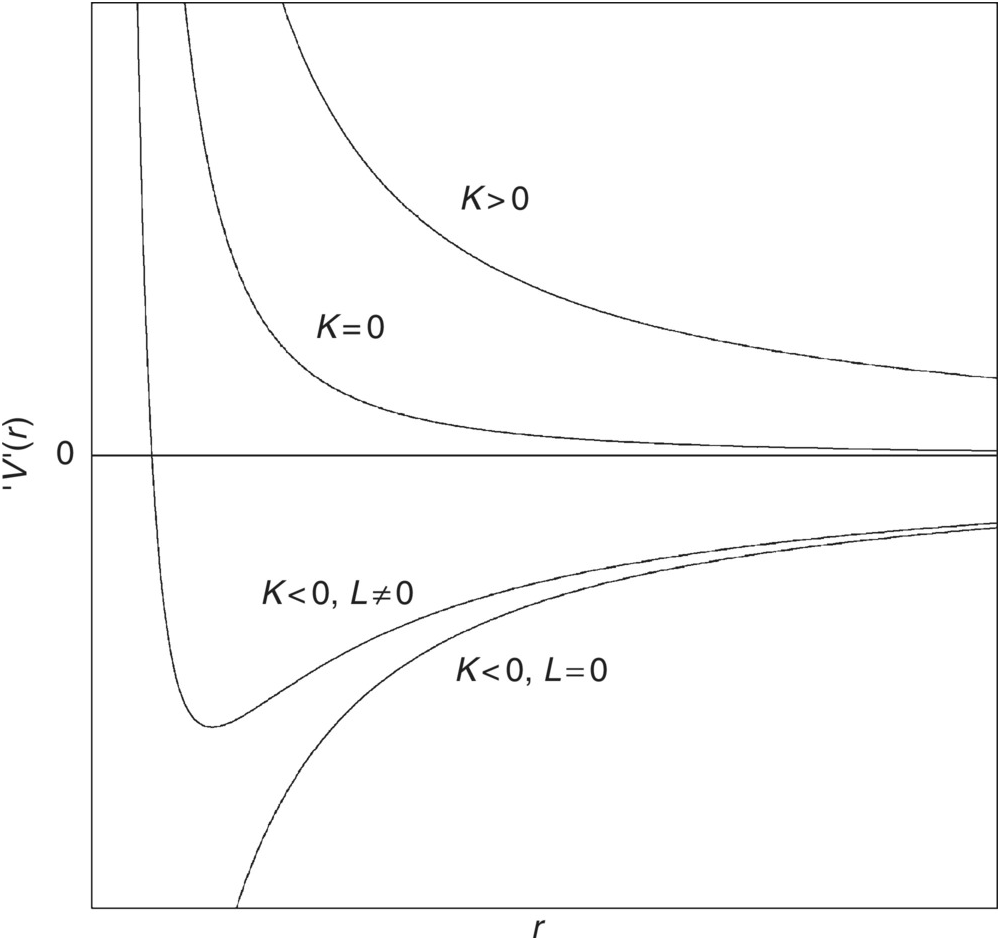
\includegraphics[scale=0.9]{fig1.png}}
\caption{The curve corresponds to $k>0$ shows repulsive inverse square force law behaviour and with $k<0$, it shows attractive inverse square force law behaviour with centrifugal barrier absent in case of $L (\quad \text{or}\quad J)=0$. Curve corresponds to $k=0$ implies that there is no central force and effective potential energy of particle is equal to its angular kinetic energy $K_{\theta,\phi}$ due to motion in $\theta$ and $\phi$ directions.}
\label{fig}
\end{figure}

 \subsection{\normalsize{\emph{\textbf{Angular Kinetic Energy $K_{\theta,\phi}$}}}}
 Velocity of particle is given by: $\vec{v} = \vec v_{\mathrm{radial}} + \vec v_{\mathrm{angular}}$, where $\vec v_{\mathrm{radial}}$ component is responsible for particle's radial kinetic energy $K_{r} = \frac{1}{2}m\dot{r}^{2} = \frac{p_{r}^{2}}{2m}$ and $\vec v_{\mathrm{angular}}$ for its angular kinetic energy $K_{\theta,\phi} =\frac{1}{2}mr^{2}(\dot{\theta}^{2} + \sin^{2}{\theta}\dot{\phi}^{2}) = \frac{p_{\theta}^{2}}{2mr^{2}} + \frac{p_{\phi}^{2}}{2mr^{2}\sin^2{\theta}} $. Thus, from (10) we can verify that $E = K_{r} + K_{\theta,\phi}$. Recall that  minimum value of energy ($E_{\mathrm{min}}$) is possible when $\dot{r} = 0$ or $K_{r} = 0$. This means for $k<0$ and $J\not=0$, we have $K_{\theta,\phi}$ at $r=r_{*}$ equals $\frac{k^{2}m}{2J^{2}}$. This means when particle has minimum energy $E_{\mathrm{min}}$, its sits at the bottom of the potential well (global minima in curve in fig1. at $r=r_{*}$) and stays there for all the time and although it has fixed radial position but it is still moving in $(\theta,\phi)$ direction with energy equals to angular kinetic energy ($K_{\theta,\phi}$) at $r=r_{*}$.
 \vspace{1em}
 
 
 
 \section{\large{\textbf{Shape of trajectory $\psi(r)$ or $r(\psi)$}}}
 Knowing about shape of trajectory of particle is crucial to get global picture about its motion and hence we want to know about shape of trajectory of particle for positive and negative values of $k$. Let $\omega = \frac{\abs{\vec v_{\mathrm{angular}}}}{r}$ be the magnitude of angular velocity ($\vec{\omega}$). To get $\omega$, we should find $\vec{\omega}$ first. Since our polar coordinates changes with time and this causes spherical unit vectors to rotate with angular velocity  $\vec{\omega}$. From eq. (5) clearly all unit vectors are independent of $r$ but depends only on $\theta$ and $\phi$. This means changing $r$ does not cause rotation of basis/unit vector but changing 
 $\theta$ and $\phi$ does and following relation holds for any unit/basis vector $\hat{e}$, \begin{dmath}\dot{\hat{e}}=\vec{\omega} \times \hat{e}\end{dmath}. Time derivatives of the unit vectors expressed in spherical coordinates are: \begin{equation}
\begin{array}{l}
\dot{\hat{r}}=\frac{\partial \hat{r}}{\partial r} \dot{r}+\frac{\partial \hat{r}}{\partial \theta} \dot{\theta}+\frac{\partial \hat{r}}{\partial \phi} \dot{\phi}=\hat{\theta} \dot{\theta}+\hat{\phi} \dot{\phi} \sin \theta \\
\dot{\hat{\theta}}=\frac{\partial \hat{\theta}}{\partial r} \dot{r}+\frac{\partial \hat{\theta}}{\partial \theta} \dot{\theta}+\frac{\partial \hat{\theta}}{\partial \phi} \dot{\phi}=-\hat{r} \dot{\theta}+\hat{\phi} \dot{\phi} \cos \theta \\
\dot{\hat{\phi}}=\frac{\partial \hat{\phi}}{\partial r} \dot{r}+\frac{\partial \hat{\phi}}{\partial \theta} \dot{\theta}+\frac{\partial \hat{\phi}}{\partial \phi} \dot{\phi}=-(\hat{r} \sin \theta+\hat{\theta} \cos \theta) \dot{\phi}
\end{array}
\end{equation}
 Let $\vec{\omega} = \omega_{r}\hat{r} + \omega_{\theta}\hat{\theta} + \omega_{\phi}\hat{\phi}$ and using (18) and (19) for all three spherical unit vectors $(\hat{r},\hat{\theta},\hat{\phi})$, we get \begin{equation}
\vec{\omega} = \dot{\phi} \cos \theta \hat{r}-\dot{\phi} \sin \theta \hat{\theta} +\dot{\theta} \hat{\phi}
\end{equation}
From (20) we have $\omega^{2} = \left[\dot{\theta}^{2}+\sin ^{2} \theta \dot{\varphi}^{2}\right]$ and from (9) we have $J = mr^{2}w$. Let $\omega = \frac{d\psi}{dt} = \sqrt{\left[\dot{\theta}^{2}+\sin ^{2} \theta \dot{\varphi}^{2}\right]} = \frac{c}{r^{2}}$, where $c$ is the specific angular momentum. This means change in angular displacement ($\psi$) is monotonic in any central-force problem and it is either continuously increasing or decreasing with $r$ with magnitude depends upon sign of specific angular momentum ($c$). If c is not zero, the independent variable can be changed from $t$ to $\psi$: \begin{equation}
\frac{dr}{d t}=\frac{dr}{d \psi}\frac{d\psi}{d t} = \frac{c}{r^{2}}\frac{dr}{d \psi}
\end{equation} 
From (21) and (14), \begin{equation}
    \frac{d\psi}{d r} = \frac{r^{2}}{c}\frac{dr}{d t} = \frac{c}{r\sqrt{ar^{2} - br - c^{2}}}
\end{equation}
Integrating (22) yields, \begin{dmath}
    \psi - \psi_{o}^{'} = \sin^{-1}{\left(A + \frac{B}{r}\right)}
\end{dmath} where $\psi_{o}^{'}$, $A = \frac{b}{\sqrt{b^{2} + 4ac^{2}}}$ and $B = \frac{2c^{2}}{\sqrt{b^{2} + 4ac^{2}}}$ are constants. Eq.(23) can be rewritten as: \begin{dmath}r = \frac{\alpha}{e\cos \left(\psi - \psi_{o}\right) + 1}\end{dmath} where $\psi_{o}$, $\alpha = -\frac{2c^{2}}{b} = -\frac{J^{2}}{mk}$ and $e = \sqrt{1 + \frac{4ac^{2}}{b^{2}}} = \sqrt{1 + \frac{2EJ^{2}}{mk^{2}}}$ are the constants. This is the equation of conic section in polar coordinates $(r, \psi)$ where $\alpha$ governs the size of the trajectory and $e$ is known as the eccentricity, governs the shape of the trajectory. Basically what we did is we convert spherical coordinates $(r,\theta,\phi)$ to polar coordinates $(r,\psi) \mid \dot{\psi} = \omega = \sqrt{\dot{\theta}^{2} + \sin^2{\theta}\dot{\phi}^{2}}$ and reduced our problem from 3D to 2D system. In this 2D system we are analyzing $r = f(t)$ and $\psi = f(r)$ which provides us the information of radial position of particle and its shape of trajectory which is different for different values of $E$ and $k$. Eq. (24) can be re-written as: $r = \frac{\alpha}{e\cos{\psi}+1}$ if we shift our point of reference ($(r = 0,\psi = 0)$ in polar coordinate system  to $(r = 0,\psi = \psi_{0})$. We did this to simplify the equation of various conic sections which we have discussed in section \RomanNumeralCaps{6}.
\vspace{1em}




\subsection{\normalsize{\emph{\textbf{Finding Relations: $t = f(\psi)$ , $\theta = f(r)$ and $\phi = f(\theta)$}}}}
Substitute $r = \frac{\alpha}{e\cos{\psi}+1}$ in expression of $\frac{d \psi}{d t}$ as follows: \begin{equation}
\begin{split}
&\frac{d \psi}{d t} = \sqrt{\dot{\theta}^{2} + \sin^{2}{\theta}\dot{\phi}^{2}} = \frac{J}{mr^{2}} = \frac{J\left(1 + e\cos{\psi}\right)^{2}}{m\alpha^{2}} \\
&\Rightarrow \frac{d \psi}{\left(1 + e\cos{\psi}\right)^{2}} = \left(\frac{mk^{2}}{J^{3}}\right) dt 
\end{split}
\end{equation}

Eq. (25) has different solutions for different values of $e$: 
\begin{equation}
\begin{split}
&\bullet \quad e=0 \Rightarrow \quad \psi = \frac{m k^{2}\left(t - t_{0}\right)}{J^{3}} \\
&\bullet \quad e=1 \Rightarrow \quad \frac{\left(\cos{\psi}+2\right)\sin{\psi}}{3\left(\cos{\psi}+1\right)^{2}} = \frac{m k^{2}\left(t - t_{0}\right)}{J^{3}} \\
&\bullet \quad e>1 \Rightarrow \quad \frac{e\sin{\psi}}{\left(e^{2}-1\right)\left(e\cos{\psi} +1\right)} \\
&-\frac{2\tanh^{-1}{\left[\sqrt{\frac{e-1}{e+1}}\tan{\left(\frac{\psi}{2}\right)}\right]}}{\left(e^{2}-1\right)^{\frac{3}{2}}} =\frac{m k^{2}\left(t - t_{0}\right)}{J^{3}}\\
&\bullet \quad e <1 \Rightarrow \quad -\frac{e\sin{\psi}}{\left(1 - e^{2}\right)\left(e\cos{\psi} +1\right)} \\
&-\frac{2\sqrt{1-e}\tan^{-1}{\left[\sqrt{\frac{1-e}{1+e}}\tan{\left(\frac{\psi}{2}\right)}\right]}}{\left(1-e\right)^{2}\left(1+e\right)^{\frac{3}{2}}} =\frac{m k^{2}\left(t - t_{0}\right)}{J^{3}}
\end{split}
\end{equation}

From expression (9), we have \begin{dmath}\dot{\theta}^{2} =  \frac{J^2}{m^{2}r^{4}} - sin^{2}{\theta}\left(\frac{p_{\phi}}{mr^{2}sin^{2}{\theta}}\right)^{2} = \frac{c^{2}}{r^{4}}\left(1 - \frac{d^{2}}{\sin^{2}{\theta}}\right)\end{dmath} 

From (14) and (27), we have \begin{dmath} \frac{c dr}{r\sqrt{ar^{2} - br - c^{2}}} = \frac{\sin{\theta} d\theta}{\sqrt{\sin^{2}{\theta} - d^{2}}}\end{dmath} where $d = \frac{p_{\phi}}{J} \left( < 1\right)$ is the constant. 
Integration eq. (27) yields, 
\begin{equation}
    \begin{split}
 &\frac{\cos{\theta}}{\lambda} = \sin{\left[r_{o} + \sin^{-1}{\left(A + \frac{B}{r}\right)}\right]} \\
 &\Rightarrow \theta = \cos^{-1}\left({\lambda\sin{\left[r_{o} + \sin^{-1}{\left(A + \frac{B}{r}\right)}\right]}}\right) \\
 &\Longleftrightarrow r = \frac{\lambda B}{M\sqrt{\lambda^{2} - \cos^{2}{\theta}} + N\cos{\theta} - \lambda A}
 \end{split}
 \end{equation} where $\lambda = \sqrt{1 - d^{2}}$ , $r_{o}$, $M$, $N$ are constants. 
Recall $\left(d\psi\right)^{2} = \left(d\theta\right)^{2} + \sin^{2}{\theta}\left(d\phi\right)^{2}$. This implies \begin{dmath}\left(\frac{d\psi}{d \theta}\right)^{2} = 1 + \sin^{2}{\theta}\left(\frac{d\phi}{d \theta}\right)^{2}\end{dmath} 
$\left(\frac{d\psi}{d \theta}\right)^{2} = \left[\frac{\left(\frac{d\psi}{d r}\right)}{\left(\frac{d\theta}{d r}\right)}\right]^{2} = \frac{c^{2}\left[g(r)\right]^{2}}{\left(\frac{d\theta}{d r}\right)^{2}}$, where $g(r) = \frac{1}{r\sqrt{ar^{2} - br - c^{2}}}$ (from (22)). Now from eq. (28) we have $\left(\frac{d\theta}{d r}\right)^{2} = c^{2}g(r)^{2}\left(1 - \frac{d^{2}}{\sin^{2}{\theta}}\right)$. Substitute this relation we get,
\begin{equation}
\left(\frac{d\psi}{d \theta}\right)^{2} = \frac{\sin^{2}{\theta}}{\sin^{2}{\theta} - d^{2}}
\Rightarrow \psi- \psi_{o} = \sin^{-1}{\left(\frac{\cos{\theta}}{\lambda}\right)}
\end{equation} where $\psi_{o}$ is the integration constant.   
Using expression obtained in (31) in eq. (30), we get \begin{dmath} d\phi =  \frac{d  d\theta}{\sin{\theta}{\sqrt{\sin^{2}{\theta} - d^{2}}}}\end{dmath} Integrating (32) yields, 
\begin{equation}
\begin{split}
&\theta = \cot^{-1}{\left[\frac{\sqrt{1 - d^{2}}}{d}\sin^{-1}{\left(\phi - \phi_{o} \right)}\right]} \\ &\Longleftrightarrow \phi - \phi_{o} = \sin{\left(\frac{d \cot{\theta}}{\sqrt{1 - d^{2}}}\right)}
\end{split}
\end{equation} where $\phi_{o}$ is the integration constant.
\vspace{1em}



\subsection{\normalsize{\emph{\textbf{Relation of $\phi$ with $r$ ($\phi = f(r)$)}}}}
Finding explicit relation among $\phi$ and $r$ is complex as there is no closed form solution of equation $\frac{d\phi}{d r} = H(r)$. Lets find the expression of $H(r)$. Since $\dot{\phi} = \frac{p_{\phi}}{mr^{2}sin^{2}{\theta}}$ which implies $\frac{d \phi}{d r} = \frac{lg(r)}{\sin^{2}{\theta(r)}}$, where $l = \frac{p_{\phi}}{m}$ (specific angular momentum about $z$ direction). Now, if we expand eq. (29) using trigonometric and inverse-trigonometric identities to get expression of $\sin^{2}{\theta}$ in terms of $r$, we get following form:  \begin{dmath}
\sin^{2}{\left[\theta(r)\right]} = \frac{k_{1}^{'}r^{2} + k_{2}^{'}r + k_{3}^{'} + \sqrt{k_{4}^{'}r^{2} + k_{5}^{'}r + k_{6}^{'}}}{r^{2}}
\end{dmath} 
This implies $H(r) = \frac{lg(r)r^{2}}{k_{1}^{'}r^{2} + k_{2}^{'}r + k_{3}^{'} + \sqrt{k_{4}^{'}r^{2} + k_{5}^{'}r + k_{6}^{'}}}$, where $k_{i}^{'} \forall{i}$ are constant. Simplifying $H(r)$ further we get, \begin{dmath} \phi(r) = C_{2} - k_{1}\int^{r}\frac{F(r) dr}{P(r^{2}) + k_{2}Q(r^{2})}\end{dmath} where $F(r) = r^{2}g(r)$, $C_{2}$, $k_{1}$, $k_{2}$ are constants and $P(r^{2})$, $Q(r^{2})$ are two degree 2 polynomials of form $r^{2} + \gamma r + \delta$ with some constant $\gamma$ and $\delta$. There is no closed form solution of eq. (35). 
\vspace{1em}




\subsection{\normalsize{\emph{\textbf{Relation of $\phi$ with $\psi$ ($\phi = f(\psi)$)}}}}
Using eq. (31), we have \begin{equation}
\frac{d \psi}{d \phi} = \frac{\dot{\psi}}{\dot{\phi}} = \frac{\sin^{2}{\theta}}{d} = \frac{1 - \lambda^{2}\sin^{2}{\left(\psi - \psi_{o}\right)}}{d}
\end{equation}
Integrating (36) yields, \begin{equation}
    \phi - \phi_{o} = \tan^{-1}{\left[d\tan{\left(\psi - \psi_{o}\right)}\right]}
\end{equation}where $\phi_{o}$ and $\psi_{o}$ are constants.
\vspace{1em}





\section{\large{\textbf{Trajectory Equations and Behaviour of Particle under Repulsive and Attractive Inverse Square Force Laws}}}
Recall the eq. of conic section in polar form, $r = \frac{\alpha}{1 + e\cos{\psi}}$. Transforming this equation into Cartesian coordinates $(x,y)$ we get following equation of conic section, \begin{dmath}\frac{(x+e \zeta)^{2}}{\zeta^{2}} \pm \frac{y^{2}}{\eta^{2}}=1 \end{dmath} $\quad \text {where} \quad e^{2}-1=\frac{2 E J^{2}}{m k^{2}}, \zeta^{2} = \frac{\alpha^{2}}{\left(1 - e^{2}\right)^{2}} , \eta^{2}=\frac{\alpha^{2}}{\abs{1 - e^{2}}} \quad\text{and}\quad \alpha = \pm\frac{J^{2}}{m\abs{k}}$. The  the \textbf{plus} sign
in the eq. (38) is for $E < 0$ and the \textbf{minus} sign for $E > 0$, whereas in $\alpha$ \textbf{plus} sign is for $k<0$ and the \textbf{minus} sign for $k>0$. 
\vspace{1em}



\subsection{\normalsize{\emph{\textbf{Trajectory Shape and Equations}}}}
From (38), it is clear that:
\subsubsection{\normalsize{\emph{\textbf{$E<0 \Rightarrow e<1$}}}} This describes an \textbf{ellipse} with semi-major axis $\zeta$ and semi-minor axis $\eta$. The center of ellipse is $(-e\zeta,0) \Rightarrow (\mp \frac{e\abs{\alpha}}{1-e^{2}},0)$ with origin (source of central potential) at distance $\frac{e\abs{\alpha}}{1-e^{2}}$ from center of ellipse. The equation will be $\frac{(x+e \zeta)^{2}}{\zeta^{2}} + \frac{y^{2}}{\eta^{2}}=1$.
\vspace{1em}



\subsubsection{\normalsize{\emph{\textbf{$E>0 \Rightarrow e>1$}}}} This describes an \textbf{hyperbola} curve with the center $(-e\zeta,0) \Rightarrow (\pm \frac{e\abs{\alpha}}{e^{2}-1},0)$ and the asymptotic lines being $y = \pm\frac{\abs{\eta} \left(x+e\zeta\right)}{\abs{\zeta}} = \pm\sqrt{e^{2}-1} \left(x+e\zeta\right)$.The equation will be $\frac{(x+e \zeta)^{2}}{\zeta^{2}} - \frac{y^{2}}{\eta^{2}}=1$.
\vspace{1em}



\subsubsection{\normalsize{\emph{\textbf{$E=0 \Rightarrow e=1$}}}} This describes a \textbf{parabola} with the equation $y^{2} = \alpha^{2} - 2\alpha x$.
\vspace{1em}



\subsubsection{\normalfont{\textbf{$E=E_{\mathrm{min}} \Rightarrow e=0$}}} This is special case in which particle radial velocity $\dot{r} = 0$ and thus the radial motion will be \textbf{uniform circular motion} with radius of circular orbit equals $r_{*} = -\frac{J^2}{km}$. This motion is possible only in case of attractive inverse square force law.
\vspace{1em}




\subsection{\normalsize{\emph{\textbf{Behaviour of Particle under Repulsive and Attractive Inverse Square Force Laws}}}}

\subsubsection{\normalsize{\emph{\textbf{Attractive Inverse Square Force Law}}}}
In this case, bounded motion is possible if $E_{\min } \leq E<0$, where $E_{\min }$ is the minimum value of $V_{\text {eff }}$. For $E \geq 0$ the radial motion is unbounded. If $E=E_{\min }$ we have a stable circular orbit. Let us now find the minimum $(r_{\min})$ and maximum distances $(r_{\max})$ for a particular energy and
angular momentum. They are given by \begin{dmath}
\begin{array}{c}
V_{\mathrm{eff}}(r)=\frac{J^{2}}{2 m r^{2}}-\frac{k}{r}=E \Rightarrow \quad E r^{2}+k r-\frac{J^{2}}{2 m}=0 \\
\Rightarrow \quad r=r_{\min , \max }=\frac{-k \pm \sqrt{k^{2}+\frac{2 E J^{2}}{m}}}{2 E} \\
=-\frac{k}{2 E}\left(1 \pm \sqrt{1+\frac{2 E J^{2}}{m k^{2}}}\right) =\beta(1 \pm e)
\end{array}
\end{dmath} where $\beta=-\frac{k}{2 E}$. Also, $E_{\min }=-\frac{mk^{2}}{2 J^{2}}(<0)$ at $r = r_{*} = \frac{J^{2}}{km}(>0)$. 
\vspace{1em}



\begin{itemize}
\item If $E<E_{\min }$, the expression inside the square root becomes negative ($e$ doesn't exist), and there is therefore no solution.
\vspace{1em}



\item If $E=E_{\min } \Rightarrow e =0$, and we have $r_{\min }=r_{\max }=\beta=\frac{J^{2}}{mk}$. This corresponds to a stable circular orbit with $r=r_{0}=\frac{J^{2}}{mk}$.
\vspace{1em}



\item If $E_{\min }<E<0 \Rightarrow e < 1$ there are two solutions, $r_{\min }=\beta(1-e), r_{\max }=\beta(1+e)$, and the
radial motion is bounded between these two distances. Notice that the shape of trajectory is ellipse in this case as $e<1$. When the orbiting particle is nearest (distance = $r_{\min}$ ) to the center then that point is called \textit{periapsis} and when it is farthest (distance = $r_{\max}$) from center then it is called \textit{apoapsis}. Moreover, the time it takes to complete one full oscillation in the radial direction, from periapsis to apoapsis and back again (also known as \textit{Time Period} $T$) is given by: \begin{dmath}
 T = 2\Delta t = T= 2\int^{r_{\max}}_{r_{\min}}\left(\sqrt{\frac{m}{2}} \frac{d r}{\sqrt{E-V_{\text {eff }}(r)}}\right)
\end{dmath}
Similarly \textit{Angular Period} ($ \Omega$), which is the angle swept out in the course of one full radial oscillation is given by: 
\begin{dmath}
\Omega = 2\Delta \psi = 2  \int^{r_{\max}}_{r_{\min}} \left(\frac{J}{\sqrt{2m}}\frac{d r}{r^{2} \sqrt{E-V_{\text {eff }}(r)}}\right) =  2\int^{r_{\max}}_{r_{\min}}\sin^{-1}{\left[\frac{1}{e} - \left(\frac{J^{2}}{\abs{k}em}\right)\frac{1}{r}\right]} \quad \text{(from $(23)$)}
\end{dmath}
\vspace{1em}



\item If $E=0 \Rightarrow e =1, \beta \to \infty$, but (39) still has a single solution at $r=r_{\min }=\frac{J^{2}}{2mk}$. There is no maximum value for $r$, so the motion becomes unbounded.
\vspace{1em}



\item If $E>0 \Rightarrow e > 1, \beta < 0 $. Since the distance $r$ must be positive, only the minus sign in (39) gives a physically acceptable solution, $r_{\min }=\beta(1-e)= \frac{\left(e-1\right) k}{2 E}$. There is again no maximum value for $r$, and the motion is unbounded. However, in this case particle trajectory is hyperbolic as $e>1$ and since $\alpha > 0 \Rightarrow r \to \infty \quad \text{when} \quad \cos{\psi} \to -\frac{1}{e}$. Since the right hand side is negative, this must occur for some angle $\psi > \frac{\pi}{2}$. This means the source of central potential is located at left side from center $(\frac{e\alpha}{e^{2}-1},0)$ of left branch of hyperbola $r = \frac{\alpha}{1 + e\cos{\psi}}$ with distance of $\frac{e\alpha}{e^{2}-1}$ between them. The right mirror branch of hyperbola is $r =\frac{\alpha}{1 + e\cos{\left(\pi - \psi\right)}} $.



\end{itemize}
\vspace{1em}



\subsubsection{\normalsize{\emph{\textbf{Repulsive Inverse Square Force Law}}}}
In this case, we have $\beta = \frac{k}{2E}$ and $e$ remains same. Unlike previous case, only unbounded motion exist in this because 
$V_{\text {eff }} >0$ for repulsive inverse square force and from (13) $E - V_{\text {eff }} >=0$ which clearly violates if $E<0$. Thus, for $E<0$ there is no motion and if $E=0$ then particle remain at rest which we already discussed in section \RomanNumeralCaps{4} A.  
\vspace{1em}


\begin{itemize}

\item If $E>0 \Rightarrow e > 1, \beta > 0 $. Since the distance $r$ must be positive, only the plus sign in (39) gives a physically acceptable solution, $r_{\max }=\beta(1+e)= \frac{\left(1+e\right) k}{2 E}$. Opposite to previous case, in this there is no minimum value for $r$, and the motion is unbounded. The trajectory shape is hyperbolic curve with center being $(-\frac{e\abs{\alpha}}{e^{2}-1},0)$ and $r \to -\infty \quad \text{when} \quad \cos{\psi} \to -\frac{1}{e}$ because sign of $\alpha$ is negative as $k>0$ in this case. However, source of central potential is located at right side from center of right branch of hyperbola $r = \frac{-\abs{\alpha}}{1 + e\cos{\psi}}$ with distance of $\frac{e\abs{\alpha}}{e^{2}-1}$ between them. The left mirror branch of hyperbola is $r =\frac{-\abs{\alpha}}{1 + e\cos{\left(\pi - \psi\right)}} $.
\end{itemize}
\vspace{1em}



\section{\large{\textbf{{Relation of $r$ with $t$ in parametric form i.e, $t = f(\rho)$ and $r = g(\rho)$ with parameter $\rho$}}}}
In this section, we will see parametric representation of eq. (14) for different values of $E$ and $k$. Parameterization provides great efficiency when differentiating and integrating curves. Parametric equations can be used to describe all types of curves that can be represented on a plane but are most often used in situations where curves on a Cartesian plane cannot be described by functions.
\begin{itemize}
\item \textbf{$k<0$ and $E<0$ :}
\begin{equation}
\begin{split}
    &\dot{r} =\sqrt{\frac{\abs{k}}{m\beta}} \frac{\sqrt{\beta^{2}e^{2} - \left(r -\beta\right)^{2}}}{r}, \quad \text{where} \quad \beta = \frac{\abs{k}}{2\abs{E}}, \\
    &e^{2} = 1 - \frac{2\abs{E}J^{2}}{m\abs{k}^{2}}
\end{split} 
\end{equation}
The solution is given by:
\begin{equation}
\begin{split}
&t -t_{o} = \sqrt{\frac{m}{\abs{k}}} \beta^{\frac{3}{2}} \left(\rho - e\sin{\rho}\right)\\
&r  = \beta\left(1 - e\cos{\rho}\right)
\end{split}
\end{equation}
\vspace{1em}

\item \textbf{$k<0$ and $E>0$ with $1<e<=\sqrt{2}$:}
\begin{equation}
\begin{split}
    &\dot{r} =\sqrt{\frac{\abs{k}}{m\abs{\beta}}} \frac{\sqrt{\left(r -\beta\right)^{2} - \beta^{2}\left(2 -e^{2}\right)}}{r}, \quad \text{where} \quad \beta = -\frac{\abs{k}}{2E}, \\
    &e^{2} = 1 + \frac{2EJ^{2}}{m\abs{k}^{2}}
\end{split} 
\end{equation}
The solution is given by:
\begin{equation}
\begin{split}
&t -t_{o} = \sqrt{\frac{m}{\abs{k}}} \abs{\beta}^{\frac{3}{2}} \left[\log{\left(\abs{\tan{\rho} + \sec{\rho}}\right)} - \sqrt{2-e^{2}}\tan{\rho}\right]\\
&r  = \beta\left(1 - \sqrt{2-e^{2}}\sec{\rho}\right)
\end{split}
\end{equation}
\vspace{1em}

\item \textbf{$k<0$ and $E>0$ with $e>\sqrt{2}$:}
\begin{equation}
\begin{split}
    &\dot{r} =\sqrt{\frac{\abs{k}}{m\abs{\beta}}} \frac{\sqrt{\left(r -\beta\right)^{2} + \beta^{2}\left(e^{2}-2\right)}}{r}, \quad \text{where} \quad \beta = -\frac{\abs{k}}{2E}, \\
    &e^{2} = 1 + \frac{2EJ^{2}}{m\abs{k}^{2}}
\end{split} 
\end{equation}
The solution is given by:
\begin{equation}
\begin{split}
&t -t_{o} = \sqrt{\frac{m}{\abs{k}}} \abs{\beta}^{\frac{3}{2}} \left[\log{\left(\abs{\tan{\rho} + \sec{\rho}}\right)} - \sqrt{e^{2}-2}\sec{\rho}\right]\\
&r  = \beta\left(1 - \sqrt{e^{2}-2}\tan{\rho}\right)
\end{split}
\end{equation}
\vspace{1em}


\item \textbf{$k>0$ and $E>0$:}
\begin{equation}
\begin{split}
    &\dot{r} =\sqrt{\frac{k}{m\beta}} \frac{\sqrt{\left(r -\beta\right)^{2} - \beta^{2}e^{2}}}{r}, \quad \text{where} \quad \beta = \frac{k}{2E}, \\
    &e^{2} = 1 + \frac{2EJ^{2}}{mk^{2}}
\end{split} 
\end{equation}
The solution is given by:
\begin{equation}
\begin{split}
&t -t_{o} = -\sqrt{\frac{m}{k}} \beta^{\frac{3}{2}} \left[\log{\left(\abs{\tan{\rho} + \sec{\rho}}\right)} - e\tan{\rho}\right]\\
&r  = \beta\left(1 - e\sec{\rho}\right)
\end{split}
\end{equation}
\vspace{1em}

\end{itemize}





\begin{comment}
\begin{table}[htbp]
\caption{Table Type Styles}
\begin{center}
\begin{tabular}{|c|c|c|c|}
\hline
\textbf{Table}&\multicolumn{3}{|c|}{\textbf{Table Column Head}} \\
\cline{2-4} 
\textbf{Head} & \textbf{\textit{Table column subhead}}& \textbf{\textit{Subhead}}& \textbf{\textit{Subhead}} \\
\hline
copy& More table copy$^{\mathrm{a}}$& &  \\
\hline
\multicolumn{4}{l}{$^{\mathrm{a}}$Sample of a Table footnote.}
\end{tabular}
\label{tab1}
\end{center}
\end{table}

\begin{figure}[htbp]
\centerline{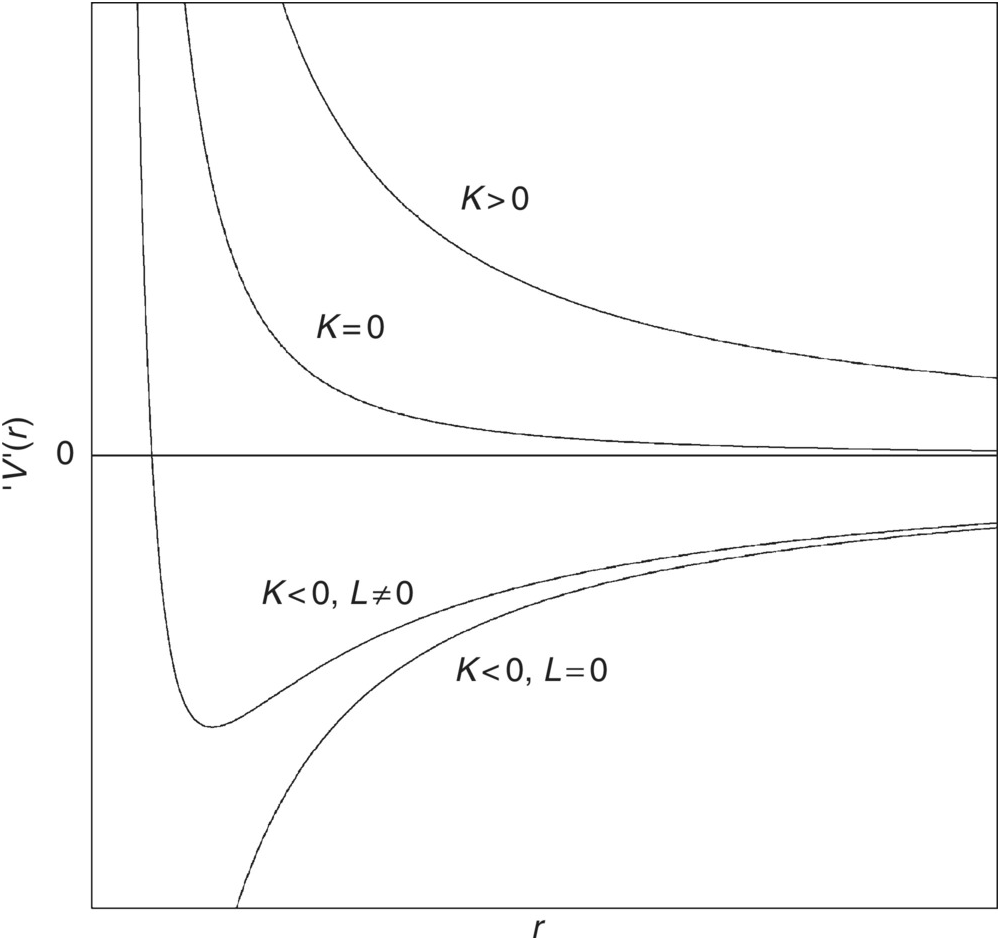
\includegraphics{fig1.png}}
\caption{Example of a figure caption.}
\label{fig}
\end{figure}


\section*{References}

Please number citations consecutively within brackets \cite{b1}. The 
sentence punctuation follows the bracket \cite{b2}. Refer simply to the reference 
number, as in \cite{b3}---do not use ``Ref. \cite{b3}'' or ``reference \cite{b3}'' except at 
the beginning of a sentence: ``Reference \cite{b3} was the first $\ldots$''

Number footnotes separately in superscripts. Place the actual footnote at 
the bottom of the column in which it was cited. Do not put footnotes in the 
abstract or reference list. Use letters for table footnotes.

Unless there are six authors or more give all authors' names; do not use 
``et al.''. Papers that have not been published, even if they have been 
submitted for publication, should be cited as ``unpublished'' \cite{b4}. Papers 
that have been accepted for publication should be cited as ``in press'' \cite{b5}. 
Capitalize only the first word in a paper title, except for proper nouns and 
element symbols.

For papers published in translation journals, please give the English 
citation first, followed by the original foreign-language citation \cite{b6}.
\end{comment}
\begin{thebibliography}{00}
\bibitem{b1} https://www.damtp.cam.ac.uk/user/tong/relativity/four.pdf
\bibitem{b2} http://www.thphys.nuim.ie/Notes/MP350/MP350-lectures.pdf
\end{thebibliography}
\end{document}
